\documentclass[10pt,twoside]{report}
\usepackage[utf8x]{inputenc}
\usepackage[english]{babel}
\usepackage{graphicx}
\usepackage[dvipsnames]{xcolor}
\usepackage[hidelinks]{hyperref}
\usepackage{lastpage,url,setspace,multicol}
\usepackage{PTSerif, PTSans}

\usepackage{geometry}
\geometry{paperwidth=215mm,paperheight=279mm,margin=20mm,outer=10mm,bottom=10mm}
\renewcommand{\baselinestretch}{.95}
\setlength{\emergencystretch}{2pt}
\setlength{\emergencystretch}{2pt}
\setlength{\emergencystretch}{2pt} % avoid some bad boxes

\makeatletter
\renewcommand*{\@oddhead}{\raisebox{0pt}[\headheight][0pt]{%
        \vbox{\hbox to \textwidth{\strut\hfil\textit{\rightmark}
\hfil\thepage}\hrule}}}
\renewcommand*{\@evenhead}{\raisebox{0pt}[\headheight][0pt]{%
        \vbox{\hbox to \textwidth{\strut\thepage\hfil%
\textit{\leftmark}\hfil}\hrule}}}
\renewcommand*{\@oddfoot}{}
\renewcommand*{\@evenfoot}{}
\renewcommand*{\chaptermark}[1]{\markboth{#1}{#1}}
\renewcommand*{\sectionmark}[1]{\markright{#1}}
\renewcommand{\thefigure}{\@arabic\c@figure}
\let\PCP=\P@Caption
\renewcommand*{\l@section}{\@dottedtocline{1}{1.5em}{2.2em}}
\newcommand{\Rmnum}[1]{\expandafter\@slowromancap\romannumeral #1@}
\renewcommand\thesection{\arabic{section}}

\renewcommand{\tableofcontents}[1][\contentsname]{%
  \thispagestyle{empty}
  \section*{#1}
  \begin{multicols}{2}
    \@starttoc{toc}
  \end{multicols}
}
\makeatother

\clubpenalty10000
\widowpenalty10000
\brokenpenalty0
\raggedbottom
\nonfrenchspacing
\renewcommand{\arraystretch}{1.6}
\columnsep2em

% Symbols
\def\D{\&}

% Chapters and sections
\def\C#1{\hypertarget{#1}{\chapter{#1}}}
\def\F#1{\hypertarget{#1}{\section{#1}}}

% Species
\newcounter{SPC1}
\newcounter{SPC2}[section]
\def\S#1{{\bigskip\noindent\textbf{\stepcounter{SPC1}\stepcounter{SPC2}\arabic{SPC2}\,(\arabic{SPC1}). #1}\par\nopagebreak[4]\medskip}}
\def\K#1{\textit{#1}}

% Photos
\setlength{\fboxsep}{2pt}
\setlength{\fboxrule}{0pt}
\def\II#1{{\nopagebreak\smallskip\raggedright\noindent\leftskip1.2em #1\par\bigskip}}
\def\I#1{\fbox{\includegraphics[width=.3\textwidth]{#1}}}

\begin{document}

\begin{titlepage}
\vspace*{\stretch{1}}
\begin{flushright}

\rule{\linewidth}{1mm}
\Huge\bfseries\sffamily
Plants of El Yunque\\[.5ex]
\huge Illustrated Checklist\\
\vspace*{1cm}
\Large\mdseries
Based on ``Flora Virtual El Verde''\\
\rule{\linewidth}{1mm}
\end{flushright}

\vspace*{1cm}
\begin{flushright}
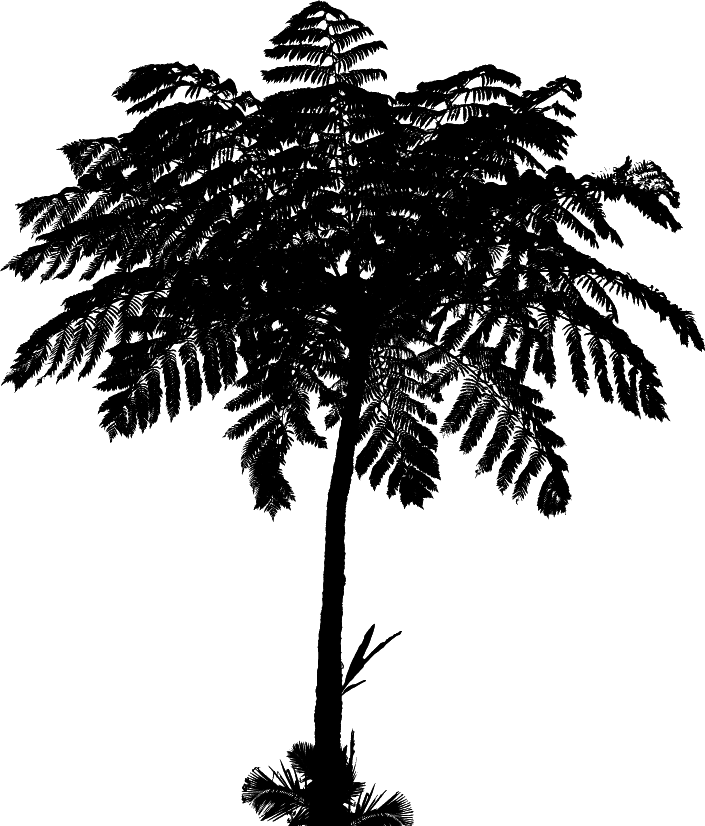
\includegraphics[width=.7\textwidth]{../../input/misc/cyathea_logo.png}\\
\end{flushright}

\hfill\small\it\today
\vspace*{\stretch{2}}
\end{titlepage}

% ===

\begin{titlepage}
\vspace*{\stretch{3}}

\noindent Plants of El Yunque. Based mostly on ``Flora Virtual El Verde'', \url{http://floraelverde.catec.upr.edu/index.php}. Version \today. \pageref{LastPage}~pp.

\vspace*{1cm}

\begin{center}
\textsl{This manual is intended exclusively for educational, non-commercial use. All rights belong to the copyright holder(s).}
\end{center}

\vspace*{\stretch{1}}

\end{titlepage}

\setcounter{page}{3}

\input body

\newpage

\tableofcontents

\end{document}
